\documentclass[english,authoryear,12pt]{elsarticle}
%%%%%%%%%%%%%%%%%%%%%%%%%%%%%%%%%%%%%%%%%%%%%%%%%%%%%%%%%%%%%%%%%%%%%%%%%%%%%%%%%%%%%%%%%%%%%%%%%%%%%%%%%%%%%%%%%%%%%%%%%%%%%%%%%%%%%%%%%%%%%%%%%%%%%%%%%%%%%%%%%%%%%%%%%%%%%%%%%%%%%%%%%%%%%%%%%%%%%%%%%%%%%%%%%%%%%%%%%%%%%%%%%%%%%%%%%%%%%%%%%%%%%%%%%%%%
\usepackage{fullpage}
\usepackage[labelfont=bf,singlelinecheck=false,aboveskip=10pt]{caption}
%\usepackage[font={scriptsize},labelfont={scriptsize},textfont={scriptsize}]{caption}
%\DeclareCaptionFormat{myformat}{#1#2\\#3}
\usepackage{amsmath,graphicx,multicol,chngpage,setspace}
\usepackage{amssymb,amsthm,amstext,amsfonts,enumerate}
\usepackage[colorlinks=true,linkcolor=black, citecolor=blue, urlcolor=blue]{hyperref}
\usepackage[top=1in, bottom=1in, left=1.0in, right=1.0in]{geometry}
\usepackage{lscape}
\usepackage{rotating}
\usepackage{color,float,multirow,array,hyphenat}
\usepackage{booktabs}
\usepackage{subcaption}
\usepackage{natbib} % already loaded by elsarticle
\usepackage{apalike}
\usepackage{babel}
\usepackage{appendix}
\usepackage{afterpage}


\setcounter{MaxMatrixCols}{10}

% Global Document settings
%\graphicspath{{C:/Work/Papers/Murray/Projects/AIT/ait-ahmad-murray/paper/Images}}
% \linespread{1.3} % Setting it to 1.3 = 1.5 line spacing; 1.6 = double spacing
\onehalfspacing
\setlength{\parindent}{0in}
\setlength{\parskip}{1em}

% Create arg max/min operator
\DeclareMathOperator*{\argmax}{arg\,max}
\DeclareMathOperator*{\argmin}{arg\,min}
\DeclareMathOperator{\E}{\mathbb{E}}

\newcommand{\bi}{\begin{itemize}}
\newcommand{\ei}{\end{itemize}}
\newcommand{\be}{\begin{enumerate}}
\newcommand{\ee}{\end{enumerate}}
\newcommand{\bd}{\begin{description}}
\newcommand{\ed}{\end{description}}
\newcommand{\prbf}[1]{\textbf{#1}}
\newcommand{\prit}[1]{\textit{#1}}
\newcommand{\beq}{\begin{equation}}
\newcommand{\eeq}{\end{equation}}
\newcommand{\beqa}{\begin{eqnarray}}
\newcommand{\eeqa}{\end{eqnarray}}
\newcommand{\bdm}{\begin{displaymath}}
\newcommand{\edm}{\end{displaymath}}
\newcommand{\script}[1]{\begin{cal}#1\end{cal}}
\newcommand{\citee}[1]{\citename{#1} \citeyear{#1}}
\newcommand{\h}[1]{\hat{#1}}
\newcommand{\ds}{\displaystyle}


% Remove Elsevier preprint message
\makeatletter
\def\ps@pprintTitle{%
	\let\@oddhead\@empty
	\let\@evenhead\@empty
	\def\@oddfoot{}%
	\let\@evenfoot\@oddfoot}
\makeatother

\begin{document}
	\begin{frontmatter}
		\title{Implications for Determinacy with Average Inflation Targeting}
		\date{\today}
		\author[1]{Yamin Ahmad}
		\ead{ahmady@uww.edu}
		\author[2]{James Murray}
		\ead{jmurray@uwlax.edu}

		\cortext[cor1]{Corresponding author}
		\address[1]{Dept. of Economics, University of Wisconsin - Whitewater, 809 W. Starin Road, Whitewater, WI 53190, USA}
		\address[2]{Dept. of Economics, University of Wisconsin - La Crosse, 1725 State St., La Crosse, WI 54601, USA}

	\date{\today}

	\begin{abstract}
		%\renewcommand{\baselinestretch}{1.5}
		In August 2020, the Federal Reserve announced a change in monetary policy behavior, where instead of targeting the inflation rate, it would target an average inflation rate over a time frame not explicitly defined. Using a calibrated three-equation New Keynesian model, We explore frameworks for combinations of backward- and forward-looking windows for an average inflation target, and investigate the conditions on the monetary policy rule for determinacy. A unique determinant equilibrium rules out an environment subject to sunspot shocks that can lead to self-fulfilling shocks to inflation expectations. We find that the length of the forward-looking window for average inflation targeting is limited to approximately three-quarters or less to assure determinacy. We further demonstrate how limitations on the length of the forward window depends on other parameters in the model, including other AIT policy parameters and parameters governing how agents form expectations.

		\begin{flushleft}
			{\it JEL Classification}: E50, E52, E58 \newline
			{\it Keywords}: Average Inflation Targeting, Determinacy, Monetary Policy, Taylor rule
		\end{flushleft}
	\end{abstract}

\end{frontmatter}

%\renewcommand{\baselinestretch}{2.0}
\renewcommand{\thefootnote}{\arabic{footnote}}%
\setcounter{page}{1}%
\setcounter{footnote}{0}%


\section{\label{Intro}Introduction}
In August 2020, the Federal Reserve became the first central bank to adopt average inflation targeting (AIT) as their monetary policy framework. At the Jackson Hole symposium, Fed Chairman Jerome Powell laid out their new strategy, under which inflation could temporarily deviate in the short run from the Fed's inflation target, as long as the average level of inflation in the medium to long run remained consistent with the Fed's target. Consequently under AIT, if inflation were to consistently remain below its target for some period, it would be followed for some period where inflation would remain above its target, and vice versa. In this way, one aim of adopting an AIT framework is to help provide a nominal anchor where long-run inflation expectations are consistent with the central bank's target.

Since the Fed's announcement, new academic research is investigating the AIT framework, examining a range of issues such as the welfare implications under AIT (e.g. \citealp{budianto2020}; \citealp{eo2020}), how adoption of AIT has affected inflation expectations (e.g. \citealp{coibion2020}; \citealp{hoffmann2022}), and the implications for boundedly-rational expectations on macroeconomic outcomes under AIT (eg: \citealp{honka2021}; \citealp{budianto2020}). A central question that pertains to the literature on the AIT framework is how the `average' level of inflation is determined. The average may be based purely on past values of inflation, expectations of future values for inflation, or some combination of the two.

We examine this issue within the context of a standard three-equation New Keynesian model. We propose a construction for an average inflation target that is a weighted average of past observations of inflation, current inflation, and expectations for the future path of inflation. We evaluate conditions on monetary policy and the inflation target window for determinacy and indeterminacy. With indeterminacy, the economy is subject to sunspot shocks, where self-fulfilling shocks to inflation expectations can lead to excess volatility in inflation and the business cycle (see, for example, \citealp{lubik2004}). To avoid excess volatility, the Federal Reserve would do well to follow a monetary policy strategy that avoids indeterminacy. This paper identifies the boundaries for average inflation targeting windows for determinate outcomes, and how these boundaries depend on the other parameters in the model.


\section{\label{Model}Model}
This paper builds upon a standard representative agent New Keynesian model along the lines of \cite{clarida1999} and \cite{steinsson2003}. This standard model consists of infinitely-lived utility-maximizing households, monopolistically-competitive firms, imperfectly flexible prices, and monetary policy.

\subsection{Baseline Framework}
There are three key equations of interest. The first is the dynamic IS curve that may be derived from the consumer's utility maximization problem. Once the model has been log-linearized, it states that the current output gap depends on expectations of the output gap next period, and is negatively related to the difference between the ex-ante real interest rate and the natural rate of interest. This is given by the equation:
\begin{equation}\label{eq:ISe}
	x_t = x_{t+1|t}^e - \frac{1}{\sigma} \left( r_t - \pi_{t+1|t}^e -r^n_t \right) + \xi_t^{x}
\end{equation}
where in period $t$, $x_t$ denotes the output gap (given by the difference between the log of output and its natural rate), $r_t$ denotes the nominal interest rate, $\pi_t$ is the inflation rate and $r^n_t$ is the natural rate of interest. The terms $x_{t+1|t}^e$ and $\pi_{t+1|t}^e$ represent time $t$ expectations of private sector agents on next period's output gap and inflation rate, respectively. The preference parameter, $\sigma$, is inversely related to consumers' intertemporal elasticity of substitution, and the shock term, $\xi_t^x$, represents a demand shock. We suppose that a fraction of agents, $\lambda\in[0,1)$, form na\"ive expectations, so that, on aggregate, expectations are given by,
\begin{equation}
	\begin{array}{c}
		x_{t+1}^e = \lambda x_t + (1-\lambda) \E_t x_{t+1} \\ [1.5pc]
		\pi_{t+1}^e = \lambda \pi_t + (1-\lambda) \E_t \pi_{t+1} \\ [1.5pc]
	\end{array}
\end{equation}
Expectations are fully rational when $\lambda=0$. We explore the implications for indeterminacy below when not all expectations are fully rational.

The second key equation is the New Keynesian Phillips Curve (NKPC), which states that inflation depends on the expectation of next period's inflation, and the output gap.
\begin{equation}\label{eq:PhillipsCurvee}
	\pi_t = \beta \pi_{t+1|t}^e + \kappa x_t + \xi_t^{\pi}
\end{equation}
where the preference parameter $\beta$ is the discount factor, $\kappa$ is a reduced form parameter that is inversely related to the degree of price stickiness, and the shock term, $\xi_t^\pi$, is a cost shock.

The third relationship is an interest rate rule that describes the conduct of monetary policy:
\begin{equation}\label{eq:TaylorRule}
	r_t = \rho_r r_{t-1} + (1-\rho_r) \left( \psi_\pi \pi_t^A + \psi_x x_t \right) + \epsilon_t^{r}
\end{equation}
where $\rho_r$ represents the parameter that central banks use to smooth the path of interest rates. The parameters $\psi_\pi$ and $\psi_x$ represent monetary policy responses to inflation and the output gap, respectively. The variable, $\pi_t^A$ represents the Fed's average inflation target. The shock term, $\epsilon_t^r$, denotes a monetary policy shock.

\subsection{Average Inflation Targeting}

Under average inflation targeting (AIT), than central bank targets an average value of inflation instead of the current inflation rate. The target window may include a backward-looking average and a forward-looking average, and the relative weights for each may be different. Suppose the average inflation target is given by,
\begin{equation}
	\pi_t^A = \gamma \pi_t^B + (1-\gamma) \pi_t^F,
\end{equation}
where $\gamma \in [0,1]$ is the relative weight given to past inflation versus expected future inflation, $\pi_t^B$ is the backward-looking average inflation, and $\pi_t^A$ is the foward-looking average inflation. We suppose that $\pi_t^B$ may be an infinitely-backward looking weighted average, where weights decline geometrically with the age of the observation. Suppose $\pi_t^B$ is given by,
\begin{equation}\label{eq:backward}
	\pi_t^B = \delta_B \pi_t + (1-\delta_B) \pi_{t-1}^B,
\end{equation}
where the weight $\delta_B \in (0,1)$ given to the most recent observation. Note that the current value for inflation, $\pi_t$, is included in this ``backward-looking" window.  Repeated substitution reveals $\pi_t^B$ the nature with which the weights declining geometrically with time,
\begin{equation}\label{eq:backward_all}
	\pi_t^B = \delta_B \sum_{j=0}^{\infty} (1-\delta_B)^j \pi_{t-j},
\end{equation}
where the weight on an observation $j$ periods in the past is given by, $\delta_B (1-\delta_B)^j$. The weights sum to one and converge to zero as observations are more distant. Smaller values for $\delta_B$ can be viewed as longer backward-looking windows for average inflation targeting. In an alternative framework with an equally-weighted mean over a finite window of $m$ periods, the weight on every observation is $1/m$. The weight of $\delta_B$ could then be thought of as approximating the monetary policy behavior of using a finite window of length $1 / \delta_B$ periods.

Similarly, suppose $\pi_t^F$ is given by,
\begin{equation}\label{eq:forward}
	\pi_t^F = \delta_F E_t \pi_{t+1} + (1-\delta_F) E_t \pi_{t+1}^F,
\end{equation}
where $\delta_F \in (0,1)$ is the weight on $E_t \pi_{t+1}$, or the weight given to the soonest expected future inflation. Note that the expression does not include the current inflation rate, which was included in the backward-looking average. The forward-looking average is a sum of only expected future outcomes. Repeated substitution of equation (\ref{eq:forward}) similarly reveals the nature the weights on future values for inflation:
\begin{equation}\label{eq:forward_all}
	\pi_t^F = \delta_F \sum_{j=0}^{\infty} (1-\delta_F)^j E_t \pi_{t+1+j},
\end{equation}
The weight given to an expected inflation rate $j$ periods in the future is equal to $\delta_F (1-\delta_F)^{j-1}$, which declines geometrically with the distance into the future. The weights converge to zero and sum to one. The weight of closest future value for inflation is given by $\delta_F$. The inverse of $\delta_F$ can be thought of as approximating the length of an equally-wighted finite forward-looking window.

The continuous nature of the forward-looking and backward-looking weighted averages are both mathematically convenient and arguably more realistic than rolling-window arithmetic mean. Equations (\ref{eq:backward}) and (\ref{eq:forward}) are difference equations over a single period. The parameters, $\delta_B$ and $\delta_F$ can be varies on a continuous scale, instead of making discrete choices for rolling window lengths. A standard Taylor-type rule, like equation (\ref{eq:TaylorRule}), is also a special case of the larger model, with $\gamma=1.0$ and $\delta_B=1.0$. By considering values for these parameters below 1.0, we can conveniently describe how AIT frameworks can differ from the standard monetary policy rule.

It may be more realistic to suppose that the central bank puts more weight on more recent past observations than on farther observations. It may be more realistic to suppose too that the central bank puts more weight on expectations for the near future than expectations for the distant future, where inflation forecasts may be less reliable. Similarly, the Fed may put more weight on more recent past inflation than on the history of inflation in the more distant past.

\subsection{Full Model}

Following \citet{sims2002}, the model can be expressed in the compact form,
\begin{equation}
	\Gamma_0 y_t = \Gamma_1 y_{t-1} + \Psi z_t + \Pi \eta_t
\end{equation}

where $y_t$ is a vector of the endogenous variables in the model, including $x_t$, $\pi_t$, $r_t$, $\pi_t^A$, $\pi_t^B$, and $\pi_t^F$; $z_t$ is a vector of the three exogenous shocks t, $\xi_t^x$, $\xi_t^\pi$, and $\xi_t^r$; and $\eta_t$ are the ex-post rational expectations forecast errors, $\eta_t \equiv y_t - E_{t-1} y_t$. \citet{sims2002} describes a method to solve the model and the conditions for existence and uniqueness (determinacy) of the solution. We use this method to explore parameter values for monetary policy behavior that lead to indeterminacy.

\begin{table}[htp]
	\captionsetup{justification=centering}
	\caption{Parameter Calibrations}\label{tb:parms}
	\begin{center}
		\begin{tabular}{lcr}
			Description & Parameter & Value(s) \\ \hline
			Discount rate (Quarterly) & $\beta$ & 0.99 \\
			Inverse intertemporal elasticity & $\sigma$ & 0.72 \\
			Phillips curve coefficient & $\kappa$ & 0.178 \\
			Monetary policy persistence & $\rho_r$ & 0.7 \\
			Monetary policy response to output gap & $\psi_x$ & 0.5 \\ [0.25pc]
			\hline \\ [-0.25pc]
			Baseline Parameters \\ \hline
			Baseline AIT weight on past inflation & $\gamma$ & $\left\{ 0.0, 0.25 \right\}$ \\
			Baseline Backward-looking weight & $\delta_B$ & 1.0 \\
			Baseline Monetary policy response to average inflation & $\psi_\pi$ & 1.5 \\ \hline
		\end{tabular}
	\end{center}
\end{table}

We calibrate the model using the parameters in \href{tb:parms}{Table} \ref{tb:parms}. In the results section below, we explore determinacy regions for different values of $\delta_F$, the weight placed on the expected value for the next period's inflation in the forward-looking window. We explore how regions of determinacy for this parameter differs with calibrations for the weight placed on past inflation in the AIT window ($\gamma$), the weight placed on the most recent inflation observation in the backward-looking window ($\delta_B$), and the Taylor rule coefficient on average inflation ($\psi_\pi$). The baseline parameters given in \href{tb:parms}{Table} \ref{tb:parms} represent the calibrations we use when not varying each of those particular parameters.

Say where I got these other parameters..

\section{Results}

\begin{figure}
	\captionsetup{justification=centering}
	\begin{center}
		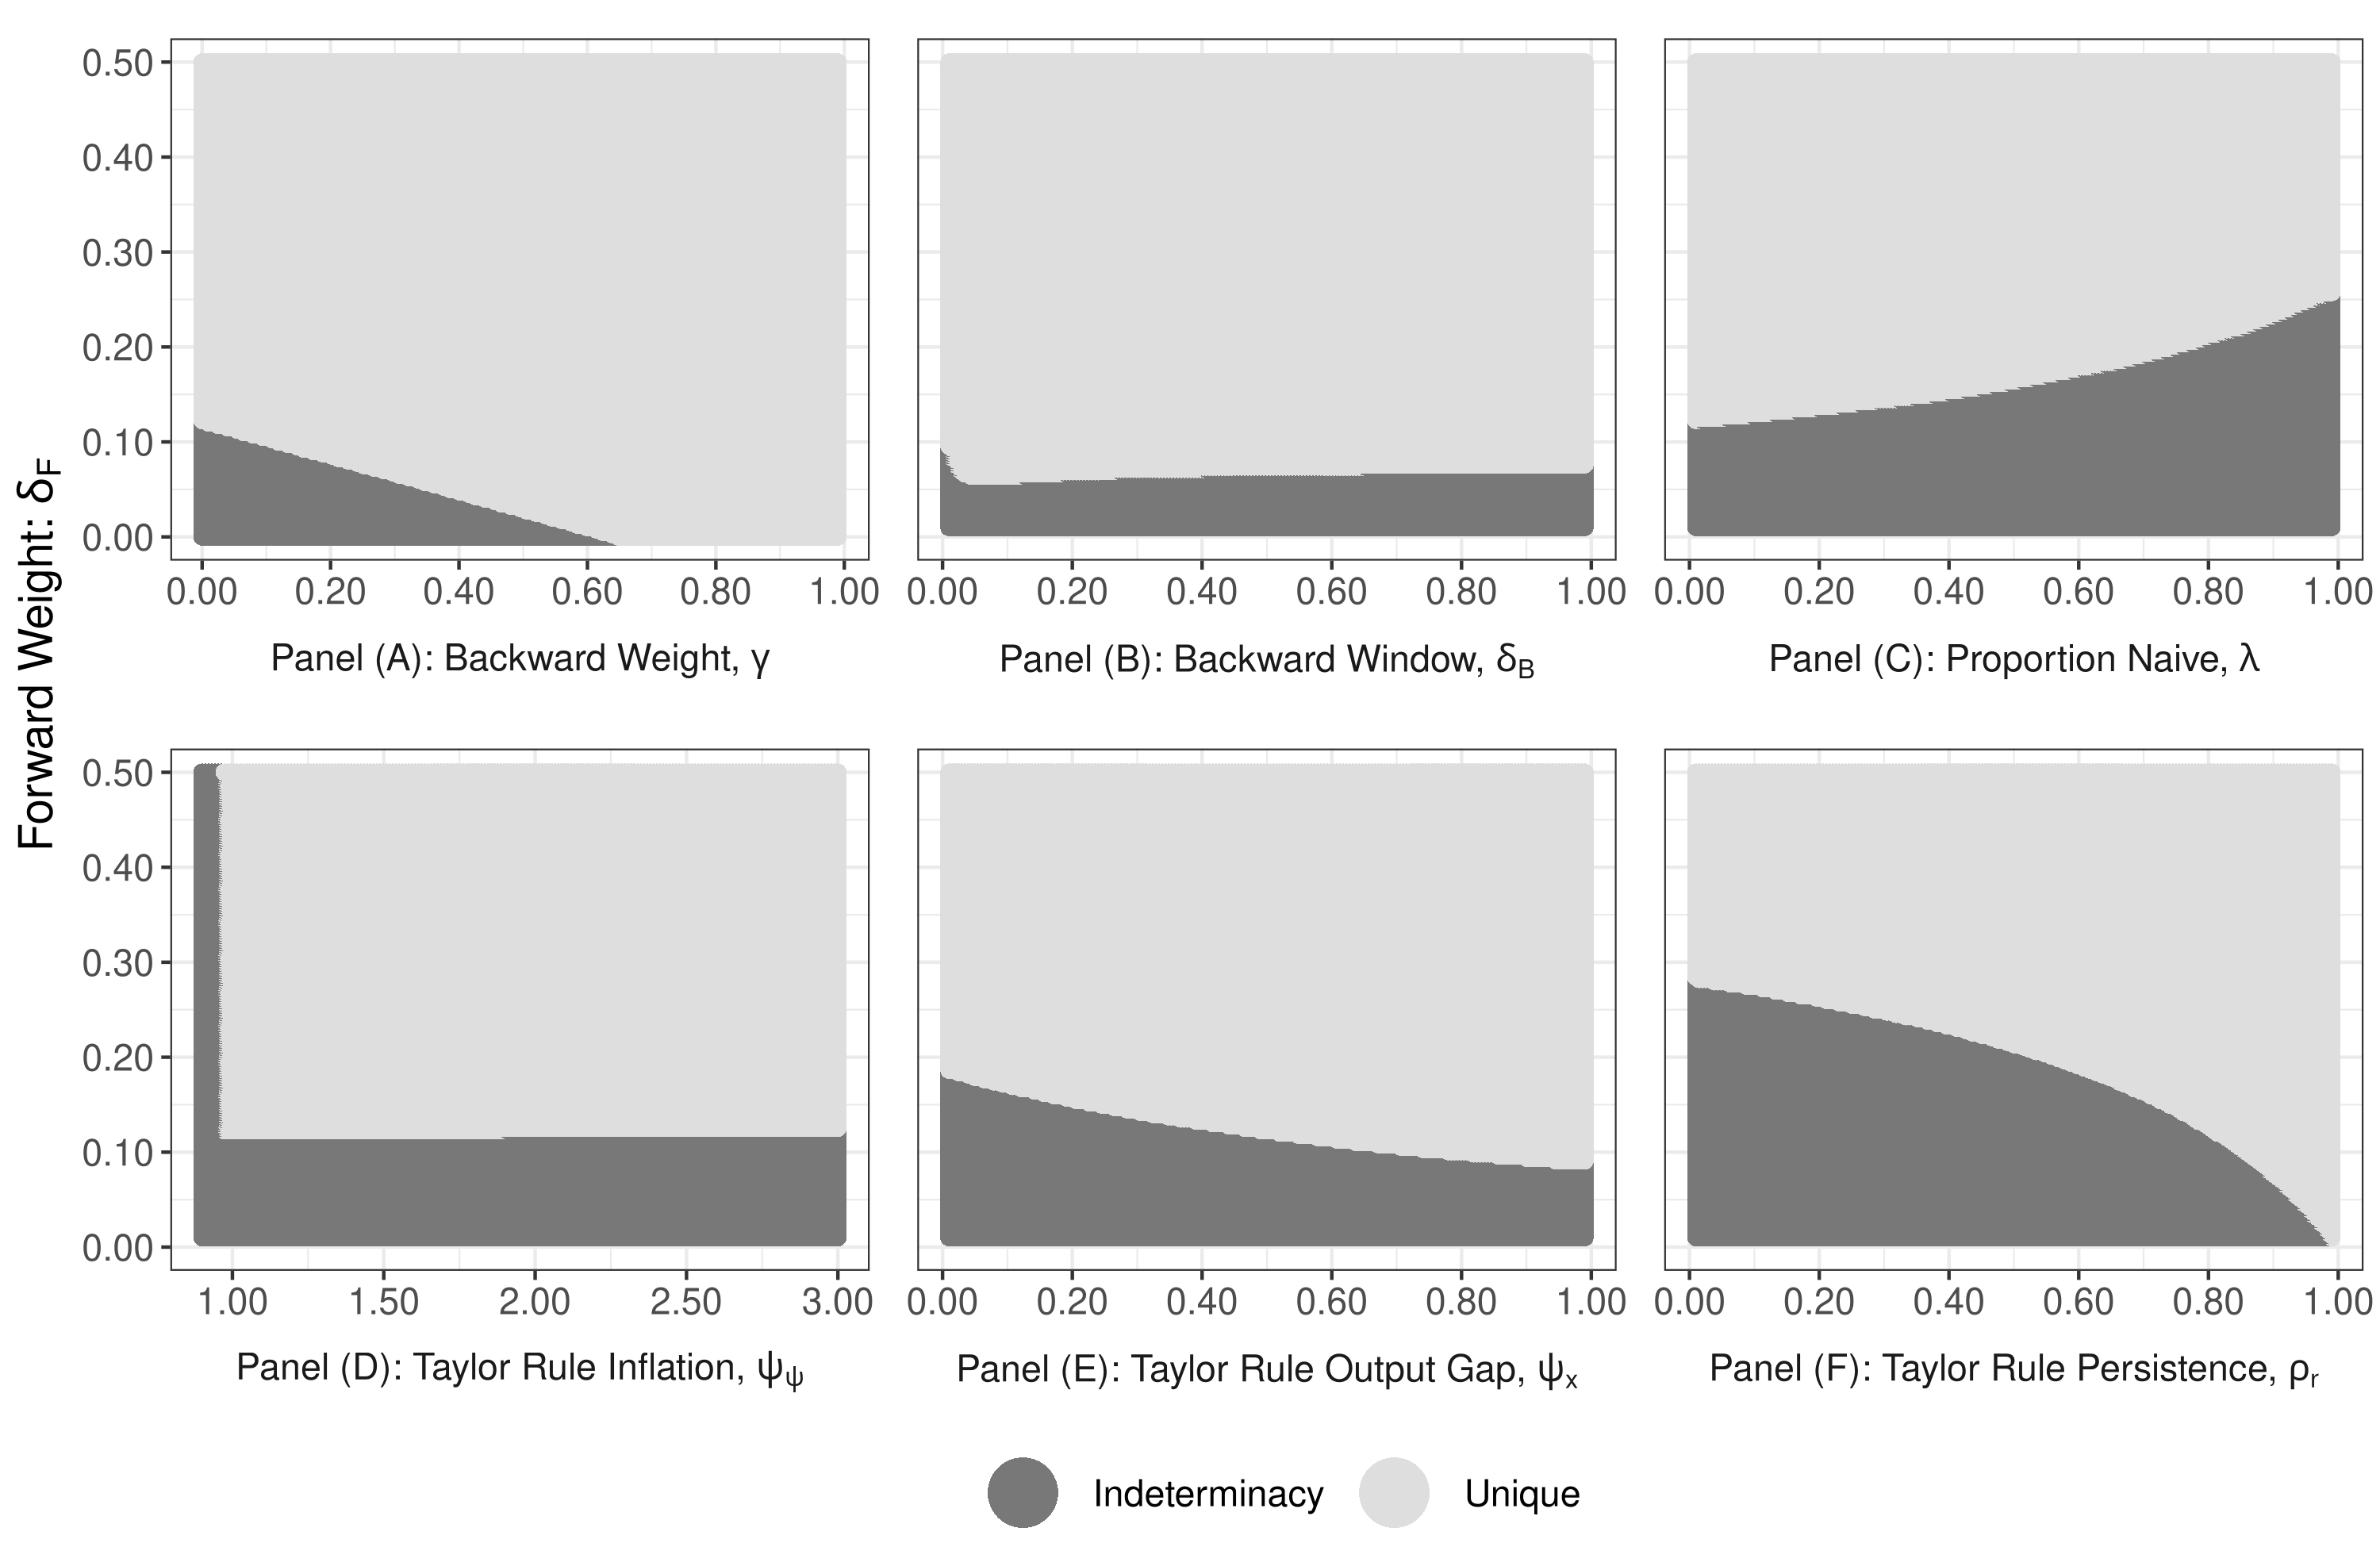
\includegraphics[width=\textwidth]{./determinacy_notitle.png}
		\ \\ \ \\
		\parbox{5.5in}{\small{
			Notes: Larger values for $\delta_F$ imply shorter forward-looking windows. Baseline values in panel (A): $\gamma=0.5$, $\lambda=0.0$, $\psi_{\pi}=1.5$; panel (B): $\lambda=0.0$, $\delta_B=1.0$, $\psi_{\pi}=1.5$; panel (C): $\gamma=0.0$, $\psi_\pi=1.5$. panel (D):  $\gamma=0.0$, $\lambda=0.0$.}
		}
	\end{center}
	\caption{Regions of Determinacy for Forward-Looking Windows}\label{fg:determinacy}
\end{figure}

\href{fg:determinacy}{Table} \ref{fg:determinacy} shows the regions of determinacy for different values of the forward-looking weight, $\delta_F$, depending on four other parameters in the model. On the vertical axis in each panel are values for $\delta_F$ from 0.0 to 1.0. Given the inverse relationship between the weight on an individual observation and the length of a finite window, can be thought of as shorter forward-looking windows. The first panel demonstrates the importance of using current or past values for inflation in the target window. When $\gamma=0.0$, no weight is put on past or current inflation, and the window is purely forward-looking. When $\gamma=0.0$, the smallest value for $\delta_F$ that delivers indeterminacy is 0.16. Taking the inverse of this value implies a forward-looking window of approximately


\bibliographystyle{apalike}
\bibliography{ait}

\end{document}
